\section{Introduction}
\label{introduction}

{\it Autonomy from human intervention in the machines that surround us promises many benefits.}
{\it Because of these benefits, autonomous and semi-autonomous systems are now an accepted part of the economy and the household.}
Examples include robots in shipping warehouses, vacuum robots and the emerging class of personal robots.
{\it Autonomous vehicles are a particularly challenging class of autonomous systems.}
{\it On a typical trip, the autonomous vehicle must recognize, enter, complete and exit many scenarios in a safe and timely manner.} 
	Example scenarios include traffic lights, roundabouts, pedestrians, weather conditions, etc. 
It is not known, ahead of time, what the specific sequence of encountered scenarios will be.

{\it The corresponding technical challenges can be broadly divided into three categories: the first is operation in a highly unpredictable environment.}
For example, what will traffic conditions be, how will other drivers behave and will they obey the laws, will certain parts of the road be inaccessible, and will there be emergency responders on the road needing right of way? 
Note that these uncertainties occur at several time scales, from the long-term (traffic conditions) to the very short-term (emergency responders driving by).
Therefore the on-board controller(s) must always decide: what is the vehicle's objective in the short run?

{\it The second challenge is that task execution must satisfy three different types of constraints: safety, comfort to the passengers and performance.}
Alternatively, these can be viewed as three objectives to be maximized.
See Fig.\ref{fig:aspects}.
\begin{figure}[tb]
	\centering
	\includegraphics{figures/placeHolder}
	\caption{Aspects of an autonomous car.}
	\label{fig:aspects}
\end{figure}
\emph{These constraints belong to different domains of analysis and are most naturally expressed and verified with different formalisms.}
How can verification results from one domain be ported over to another domain, so a coherent view of the system's operation arises?
{\it In particular, the safety of the car's passengers and of the people in its immediate environment, is imperative at all times.}
{\it Because of its importance, guaranteeing safety to a socially acceptable degree requires formal guarantees.}
Potential legal repercussions of autonomous car accidents make such guarantees even more pressing.
Thus it is essential to understand: what does safety mean in a given driving situation?

The third challenge is that there is a wide separation between the highest levels of plan execution ("go from A to B") and the lowest levels of plan execution ("accelerate steadily for the next 5 seconds"). 
How do we guarantee consistency between the commands issued at the different levels?
The most common approach to dealing with this \emph{execution abstraction stack} is to perform a corresponding separation of the control objectives and design separate controllers for each layer \cite{UrmsonX07_Tartan}. See Fig.\ref{fig:tartanHierarchy}.
\begin{figure}[tb]
	\label{fig:tartanHierarchy}
	\includegraphics[scale=1]{placeHolder.pdf}
	\caption{The execution abstraction stack and corresponding typical control hierarchy for autonomous navigation.}
\end{figure}

{\it Today we have theories that deal with \emph{high-level planning in a discrete grid world} (see Fig.\ref{fig:discreteview}), determining which `box' the car should go to given what boxes are occupied by the other vehicles, and given non-deterministic descriptions of their behaviors in Linear Temporal Logic(LTL).
}
E.g., \cite{WongpiromsarnTM10hscc,RamanK13_ImpossibleBehaviors}.
We note that these controller synthesis algorithms suffer from a doubly-exponential computational complexity \cite{PnueliR89}, though polynomial complexity algorithms exist for a fragment of LTL \cite{KleinP10_RevisitingGR1}.
{\it We also have methods for verification of temporal logic properties of the closed-loop system} modeled as some kind of finite automaton, e.g., \cite{Bouyer06latin}.
\begin{figure}[tb]
	\label{fig:discreteview}
	\includegraphics[scale=1]{placeHolder.pdf}
	\caption{Discrete view of the world for the planning controller. The road is a grid with binary occupancy in each box, and the closed-loop system (car + controller) is given by a finite automaton.}
\end{figure}
{\it At the other end of the abstraction spectrum, control theory provides analysis and design tools of low level controllers. Automatic analysis tools exist \cite{KloetzerB08tac} but are limited in scope.}
See, e.g., \todo[inline]{Sriram's Lyap from simulations, Geir Dellerud's STORMED hybrid systems, decidable classes of HS}, or provide probabilistic guarantees of completeness \todo[inline]{GF's staliro}.
{\it Because of the large degree of unpredictability, compute- and memory-intensive low level methods can't be used alone (let alone manual methods). }

The gap between high-level grid world as we will call it, and the low-level physical world is two-fold:
first, high-level synthesis and verification algorithms apply to the grid world  and to model representations that bear no a priori connection to the most accurate models of the system that we have, namely, the models of the continuous dynamics and of the code controlling them.
Secondly, the verification effort at the low-level is unaware of the commands that will be issued at the high level. 
{\it To bridge the gap between the high-level planning and verification methods, and the lower-level control-theoretic analysis tools, guaranteed abstractions have been proposed.}
Given a representation of a system, e.g. as a system of differential equations, a guaranteed abstraction of that system produces a second representation which is simpler, and yet whose external behavior is similar, in a certain precise sense, to that of the original system.
Some of these abstractions produce finite-state systems ???h. tanner, tabuada, which are amenable to model checking [???Principles of MC]. 
Others result in lower-dimensional (but still infinite-state) systems [???girard, julius, Mahesh Vishwanathan and IMEAD pabithra], for which some verification techniques are better suited.
Yet, the conditions under which these abstractions can be obtained restrict their application when it comes to industrially developed systems, where the system is conceptually decomposed into different \emph{aspects}, each of which is developed and tested by a different team.


%Typically, a CEGAR loop \todo[inline]{Clarke JACM} is required to guarantee completeness of the verification algorithm. 
	
Because of the safety imperative, we can't rely on non-guaranteed abstractions.  
	In this paper, we demonstrate the need for using multiple formalisms in the verification of autonomous plans. 
	We illustrate this with a case study of a typical lane change maneuver.


\begin{exmp}[Lane Change 1]
	\todo[inline]{change to Lane change 1,2,...}
	We use a passing scenario as a running example.
	The scenario shows the ego vehicle driving in the right lane of a uni-directional two lane road network. 
	Another car is driving in front of the ego vehicle at a lower speed.
	The ego vehicle's planner decides to initiate a passing maneuver, which involves moving to the left lane, accelerating to pass the other vehicle, then moving back into the right lane ahead of the other vehicle.
	The scenario terminates with an intersection governed by a traffic light. 
	The safety requirement is that the ego vehicle must remain at least a certain distance away from the other vehicle.
	The mission goal is to arrive at and cross the intersection.
	The verification engineer is given a vehicle controller and must check formally that the closed-loop system (ego vehicle + controller), in the representation used by the controller, performs correctly and safely.
	E.g., that representation can be a finite automaton, and the road is represented by a finite grid.
	Thus model checking will happen on this finite representation.
	Yet the safety requirement requires us to work with the more accurate continuous dynamics to determine the cars' movements during a lane change, especially during lateral changes of position. 
	Thus we need both model checking techniques, and reachability computations, to verify the safe and correct completion of this scenario.
	From a planning perspective we define the safety of the discrete controller of the target vehicle to be the satisfaction of the following safety and liveness properties:
	\begin{enumerate}
		\item The target vehicle may not exceed the speed limit (safety).
		\item The target vehicle may not collide with any other vehicles (if they exist) on the road (safety).
		\item The target vehicle must stop at a red light (safety).
		\item The target vehicle must eventually complete the scenario (liveness).
		It is possible to specify these properties using LTL operators (always and eventually).
	\end{enumerate}
\end{exmp}



%Work on autonomous navigation: DARPA urban challenge papers, controller synthesis papers.
%
%DSL: that paper by the french authors, others?
%
%Scenarios and agents: there has to be a tonne here...the papers referenced by Matt in the APEX preso
%
%Interaction between model checkers and other verif tools: CEGAR, matthias and CMU guy, spaceex.
%
% HASTEN
%
%Other semi-formal verif: staliro, breach, apx bisimulations.

\subsection{Notation}
We denote the set of integers including 0 with $\Ne$. 
Given a subset $S$ of the reals, $S^* = S \setminus \{0\}$ and $S_+ = S \cap [0,\infty)$,
while $S_+^* = S \cap (0,\infty)$.
A \emph{discrete} variable takes values in a finite set, and a \emph{continuous} variable takes values in a closed subset of $\reals^n$ for some $n$.
Given a vector $x = (x_1,\ldots,x_n) \in \reals^n$, and a set of indices $V \subset \{1,\ldots,n\}$, $\proj{x}{V}$ is the projection of $x$ onto the subspsace whose dimensions are indexed by $V$. 
E.g. with $x = (x_1,x_2,x_3,x_4)$ and $V=\{1,3\}$, $\proj{x}{V} = (x_1,x_3)$.
We also define $x^\uparrow \defeq \proj{x}{V}^{-1}$ when $V$ is clear from the context.
A set-valued map $F: \reals^n \rightrightarrows \reals^m$ maps each $x$ in its domain to a subset of its range.
For a set $K \subset \reals^n$, we abuse notation by writing $F(K)$ for $\cup_{x\in K}F(x)$.